\chapter{Validation}
In this chapter we will consider how to validate and compare different models, dealing with hyperparameters choice and with under/overfitting problem.

Bias-Variance decomposition provides an useful framework to understand the validation issue, showing how the estimation of a model performance is difficult and 
considering also the role of different training set realizations: it show again the need of a trade-off between fitting capability (bias) and model flexibility (variance) in different way.

\begin{figure}
	\caption{Behaviour of test sample and training sample error as the model complexity is varied}
	\label{img:biasVariance}
	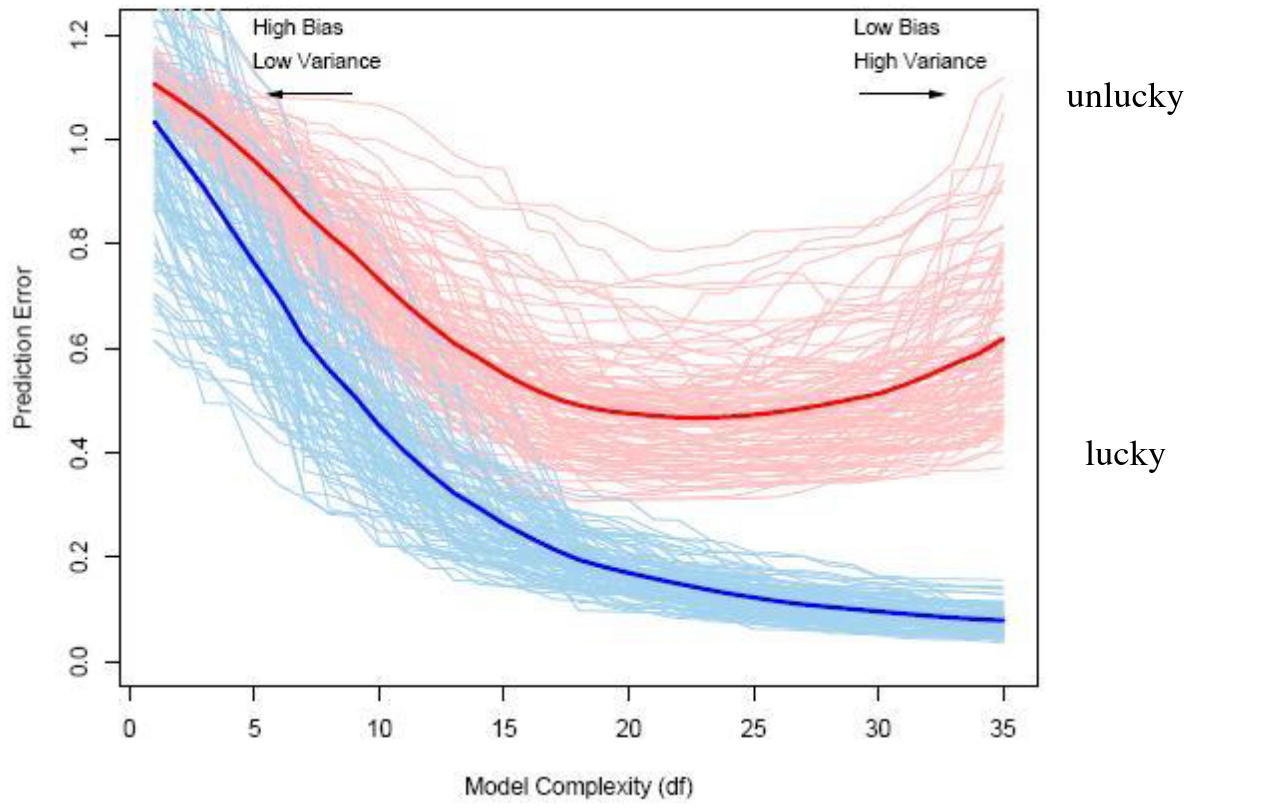
\includegraphics[width=\textwidth]{images/biasVariance}
\end{figure}
We are looking for the best solution (minimal test error), searching a balancing between fitting (accuracy on training data) and model complexity and we have that training set is 
not a good estimate of test error: initially it has too many bias (under fitting, high TR error) than too high variance (low TR error but over fitting),
as you can note in figure \ref{img:biasVariance}.\newline
Assuming a tuning parameters $\theta$ (implicit or explicit) that varies the model complexity, we wish to find the value of  $\theta$ that minimizes test error and 
we are looking for methods for estimating the expected  error for a model.

We can do an analytically validation using AIC/BIC (Akaike/Bayesian Information Criterion, limited to linear models), MDL and SRM (Structural Risk Minimization and VC-dimension), but 
in practice, often we can approximate the estimation on the data set: by resampling (direct estimation of extra-sample error via cross-validation or via bootstrap).

Validation has $2$ aims:
	 \begin{enumerate}
	    \item \emph{Model selection} where we estimating the performance (generalization error)
		  of different learning models in order to choose the best one (to generalize) and 
		  this includes search the best hyper-parameters of your model and returns a model.
	    \item \emph{Model assessment}, after we have chosen a final model,
		  estimating/evaluating its prediction error/ risk (generalization error)
		  on new test data (measure of the quality/performance of the ultimately chosen model)
		  and it returns an estimation.
	 \end{enumerate}
	 A good rule is to keep a separation between goals and use separate datasets to validate
	 and test our model, so we should have $3$ dataset: a training set, to find the best 
	 hypothesis, a validation set for model selection and in the end a external unseen 
	 test dataset to estimate our prediction error.
	    
	 If we have infinite data there are not problem, but we have only a small amount of data
	 we have to choose how to create these $3$ datasets so we present now some technique
	 to do validation, that will be extended later during the course:
	 \begin{description}
	     \item [Hold-out Cross Validation: ] we partition dataset $D$ into $3$ disjoint sets
		    training set $TR$, validation set $VL$ and test set $TS$, as we can see
		    in figure \ref{img:hold-out} and in figure \ref{img:dataset} we can see
		    the purpose of each dataset.
	     
	    \item [K-fold Cross Validation: ] Hold CV make an insufficient use of data so we 
		  split the dataset $D$ (note figure \ref{img:k-fold}) into $k$ mutually exclusive subsets $D_1, D_2, \dots, D_k$
		  to train the learning algorithm on $D - D_i$ and test it on $D_i$ and it uses
		  all the data for training and validation/testing.
		  You don't get an unique model, but you get also a variance over different folders for your class of models/algorithms.
	\end{description}

	\begin{figure}
	    \caption{Representation of dataset in Hold-out validation}
	    \label{img:hold-out}
	    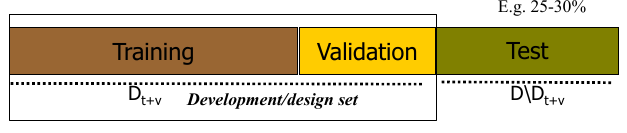
\includegraphics[width=\textwidth]{images/holdOut}
	\end{figure}
	
	\begin{figure}
	    \caption{Purpose of Training, validation and testset}
	    \label{img:dataset}
	    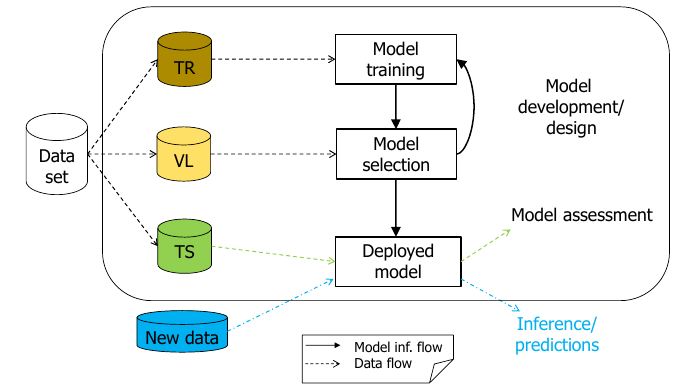
\includegraphics[width=\textwidth]{images/dataSet}
	\end{figure}

	\begin{figure}
	   \caption{Representation of dataset in K-fold Cross Validation}
	   \label{img:k-fold}
	   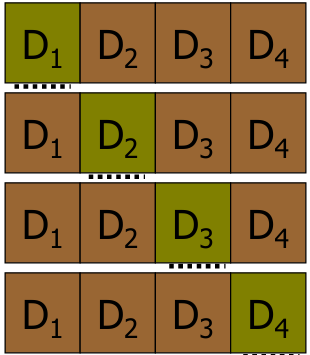
\includegraphics[width=\textwidth]{images/kfold}
	\end{figure}
	We define as validation metrics to consider the following:
	\begin{itemize}
	    \item Specificity define as $TN / (FP + TN)$ where $TN$ are true negative and $FP$ are false positive.
	    \item Sensitivity define as $TP / (TP + FN)$
	    \item Accuracy define as $TP + TN / total$
	    \item ROC curve: in figure \ref{img:roc} it is possible to discover the ROC curve where the diagonal corresponds to the 
		  worst classificator and better curves have higher AUC (Area Under the Curve).
	\end{itemize}

	\begin{figure}
	    \caption{ROC Curve Phenomena}
	    \label{img:roc}
	    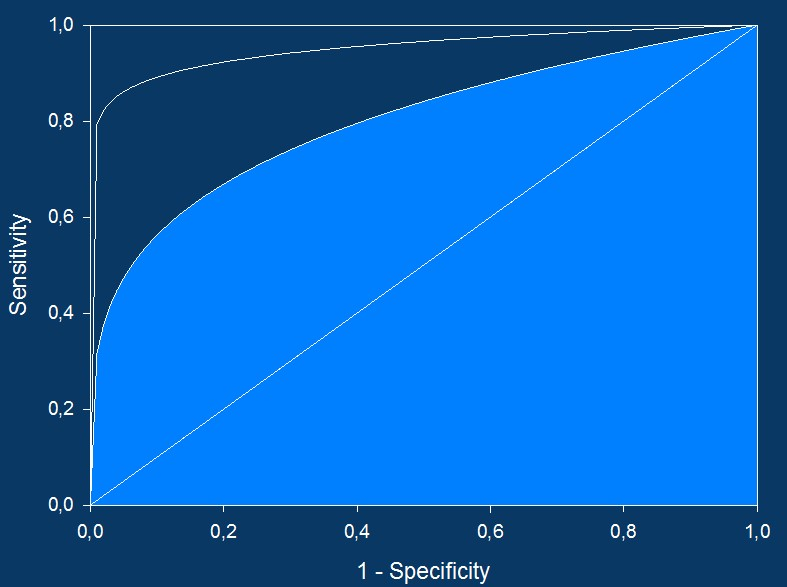
\includegraphics[width=\textwidth]{images/rocCurve}
	\end{figure}

	\emph{Grid search} (model selection phase) permits to choose value of Hyperparameters, parameters that are not directly learnt within estimators, that can be set by searching 
	a hyperparameters space (of course by model selection on a validation set) and \emph{Exhaustive Grid Search} exhaustively generates candidates from a grid of parameter values,
	and can be automatize it, where parallelization is easy with independence of trials, but the cost of search can be high (Cartesian product between the sets of values for each hyperparameter)
	and can be useful to fix some hyperparameters values in a preliminary experimental phase (since they show to be not relevant).\newline
	We can have two (or more) levels of grid search: apply a first coarse grid search to the (other) hyperparameters with a  table on the combinations of all the possible
	(growing exponential) values too find good intervals (regions) and then a finer grid-search can be performed over smaller interval and with selected hyperparameters.

	\emph{Bootstrap} is the random resampling with replacement and repeat it to form different subsets (vd or  ts) and we have again an important rule:
	Keep separation between goals and use separate sets (TR for training, VL for model selection,  TS for risk estimation).


